\documentclass{article}


\usepackage[utf8]{inputenc} % allow utf-8 input
\usepackage[T1]{fontenc}    % use 8-bit T1 fonts
\usepackage{hyperref}       % hyperlinks
\usepackage{url}            % simple URL typesetting
\usepackage{booktabs}       % professional-quality tables
\usepackage{nicefrac}       % compact symbols for 1/2, etc.
\usepackage{microtype}      % microtypography
\usepackage{amsmath,amsthm,amsfonts,amssymb,amscd}
\usepackage{tikz}
\usetikzlibrary{arrows, automata, shapes, bayesnet}
\usepackage{dsfont}
\usepackage{algorithm}
\usepackage{algpseudocode}

\usepackage{float}
\usepackage{subcaption}
\usepackage{hyperref}
\usepackage[final, nonatbib]{nips_2016}

\title{Protein Contact Prediction with Three-way CRF Factors}
\date{December 20, 2016}
\author{Roshan Rao and Edward Williams}

\begin{document}
\maketitle

\section{Introduction}
\vspace*{-0.1in}
Protein structure prediction is a seminal problem in computational biology. The goal of protein structure prediction is to infer the 3D structure of a protein from its amino acid sequence. Previous work in this field generally uses simulated annealing to determine protein structure, however Pacheco et. al. are currently attempting to apply the D-PMP algorithm, which had success in the sub-problem of protein side chain prediction, to full structure prediction. D-PMP is a dynamic programming algorithm that operates on pairwise Markov Random Fields (MRFs). A protein can be represented as a pairwise MRF by assigning a variable to each amino acid to keep track of its position and orientation, and adding an edge between variables if the corresponding amino acids are close enough to interact. 

In order to obtain efficient inference for D-PMP it is necessary to provide a sparse graphical model. Currently, D-PMP is being provided with the true graph structure, obtained using knowledge of the correct protein structure. Note that the complete graph is always a valid representation of a protein, but this requires high computational cost. However, although inter-atomic energies never vanish, they do have an inverse square relationship with distance. Therefore it is computationally beneficial to remove edges between amino acids that are beyond some specified interaction distance, and thus have inter-atomic energy near zero. On the other hand, removing edges between amino acids that are within that interaction distance can significantly impact energy evaluation and cause inference to fail. Seen in this manner, the problem of predicting a sparse graph structure is equivalent to determining the probability that two amino acids will be within the interaction distance in the final protein structure, with a goal of limiting false negatives. Here we describe a CRF-based method for estimating the adjacency matrix of a protein given its amino acid sequence, a problem known as protein contact prediction.
\section{Related Work}

Predicting amino acid contacts is an active area of research in the field of protein structure prediction. An accurate adjacency matrix for a protein's 3D structure is useful for two applications: initializing a protein structure prediction algorithm, and using the amino acid contacts to predict 3D structure directly. An accurate set of protein contacts reduces the number of pairwise interactions that must be calculated when predicting 3D protein configuration with an energy model. This reduces the computational load, speeding up execution time \cite{wuyun16}. 
Efforts to predict a 3D protein structure \emph{de novo} by using amino acid proximity estimates to constrain structure have proven partially successful, with an RMSD error range of 2.7-5.1 \AA{} across 75\% of the protein chain for proteins with 50-260 amino acid residues \cite{colwell11}.
\\ Rather than attempting to predict amino acid contacts from an amino acid sequence directly, modern contact prediction algorithms have relied on relationships between homologous protein domains, which are subdivisions of proteins that are evolutionarily related. Ekeberg et al. use sequence-aligned protein domains to fit a Potts model to protein domain families \cite{ekeberg13}. The Potts model, learned via pseudolikelihood maximization, contains a set of coupling strengths between amino acid pairs at particular positions in the amino acid chain, and is used to produce a contact map. In this model, amino acid positions in a sequence are likely to be in contact if their values are correlated across many proteins domains in the sequence's family. Other approaches model protein families as Gaussian Graphical Models with some correlations existing between families \cite{ma15}. Unfortunately, protein domain family models, such as the Potts model presented by Ekeberg et al., tend to produce many false negatives in their final predictions. As mentioned above, false negatives are much more detrimental to D-PMP inference than false positives. The CoinFold contact prediction system \cite{wang16}, combines evolutionary correlation models,  sequence-level features, and some elements of 3D structure prediction, which may produce a model more uniquely suited to initializing a physical protein structure prediction algorithm. However, the CoinFold model still focuses on minimizing total error and obtains a large number of false negatives. As well, attempting to predict the 3D structure of a protein using a model initialized with a different structure prediction system may produce spurious results. 
\\ A paper recently presented by Golkov et al. at NIPS provides a close analogue to our stated goal of initializing a protein, although they use an co-evolutionary Potts model technique. Golkov et al. use the results of the Potts model to train a convolutional neural network to predict contact maps. This method outperforms the contact prediction technique presented by Ekeberg et al., as it the convolutional neural network architecture can use amino acid pairs' neighbors to inform prediction \cite{golkov16}. 


\section{Model}
Let $y_1, y_2, \ldots y_N$ represent the observed amino acid sequence of a protein. Each variable $y_i$ denotes the type of amino acid at the $i$-th position in the sequence. Our goal is to predict a symmetric adjacency matrix $X$:
\begin{equation} \label{eq:adjmatrix}
\mathbb{P}\Bigg(
\begin{bmatrix} 
0         & x_{12} & x_{13} & \dots   & x_{1N} \\
x_{12} & 0         & x_{23} & \dots   & x_{2N} \\
x_{13} & x_{23} & 0         &            &             \\
\vdots & \vdots  &            & \ddots & \vdots   \\
x_{1N} & x_{2N} &          & \dots    & 0
\end{bmatrix}
\Bigg| \; y_1, \ldots, y_N\Bigg) 
\end{equation}
where entry $x_{ij} = 1$ if the corresponding amino acids $y_i, y_j$ are within the specified interaction distance. We do this by extracting features from the amino acid sequence and creating an exponential family model, which we represent using a conditional random field (CRF). 
\subsection{Features}
We use three features extracted from the observed sequence $y$ along with a three-factor interaction feature between variables $x_{ij}, x_{ik},$ and $x_{jk}$. The sequence features are a distance feature $\phi_{\textmd{dist}}(y_i, y_j) = |i - j|$, a sequence length feature $\phi_{\textmd{seqlen}}(y) = N$ (which acts as a prior), and amino acid pair features. The amino acid pair features are defined as follows: let $A, B$ be two types of amino acids. Then $\phi_{A, B}(y_i, y_j) = \mathds{1}\{y_i = A, y_j = B\}$, with $\phi_{A, B} = \phi_{B, A}$. Since there are 20 total types of amino acids, this creates 210 distinct indicator variables.

Additionally we note that $\mathbb{P}(x_{ij} \mid x_{ik} = 1, x_{jk} = 1) > \mathbb{P}(x_{ij})$. This leads to triplet factors $\phi_2(x_{ij}, x_{ik}, x_{jk}) = \mathds{1}\{x_{ij} + x_{ik} + x_{jk} = 2\}$ and $\phi_3(x_{ij}, x_{ik}, x_{jk}) = \mathds{1}\{x_{ij} + x_{ik} + x_{jk} = 3\}$. 
% Add graph of this maybe?
\subsection{Graphical Model}
The full log-likelihood is then given by
\begin{multline} \label{eq:likelihood}
\mathcal{L}(y, \theta) = \exp\bigg\{\sum_{i, j} x_{ij}\bigg[\theta_{\textmd{dist}}|i - j|+ \theta_{\textmd{seqlen}}N + \sum_{A, B} \theta_{A, B}\mathds{1}\{y_i = A, y_j = B\}\bigg] \\
\sum_{i, j, k}\Big(\theta_2\mathds{1}\{x_{ij} + x_{ik} + x_{jk} = 2\} + \theta_3\mathds{1}\{x_{ij} + x_{ik} + x_{jk} = 3\}\Big)  - \Phi(y, \theta) \bigg\}
\end{multline}

This likelihood then factorizes into the graphical model depicted in Figure \ref{fig:model} below.
\begin{figure}
\centering
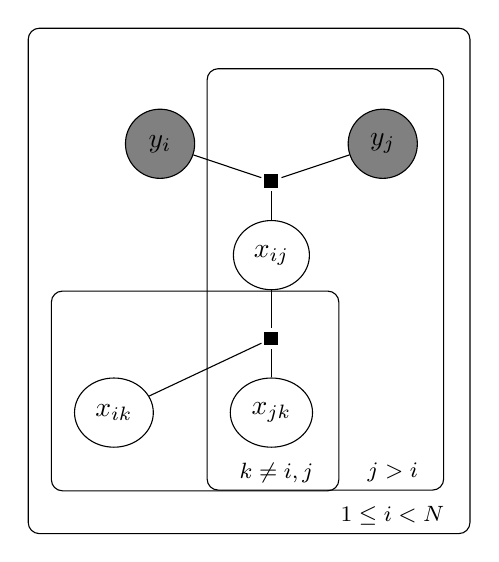
\begin{tikzpicture}[-, >=stealth', shorten >=1pt, auto, node distance=2cm, every state/.style={fill=white, draw=black, text=black, ellipse, align=center}]
	\node[state] (xij) {$x_{ij}$};
	\node[state, fill=gray] (yj) [above right of=xij] {$y_j$};
	\node[state, fill=gray] (yi) [above left of=xij] {$y_i$};
	\node[state] (xjk) [below of=xij] {$x_{jk}$};
	\node[state] (xik) [left of=xjk] {$x_{ik}$};
	\factor[above =of xij] {appearance-f} {} {} {};
	\factor[above=of xjk] {edge-f} {} {} {};
	
	\factoredge {xij} {appearance-f} {} ;
	\factoredge {yi} {appearance-f} {} ;
	\factoredge {yj} {appearance-f} {} ;
	\factoredge {xij} {edge-f} {} ;
	\factoredge {xjk} {edge-f} {} ;
	\factoredge {xik} {edge-f} {} ;
		
	\plate [inner sep=.3cm,xshift=.02cm,yshift=.2cm] {platek} {(xik)(xjk)(edge-f)} {$k \neq i, j$};
	\plate [inner sep=.3cm,xshift=.02cm,yshift=.2cm] {platej} {(xij)(yj)(xjk)} {$j > i$};
	\plate [inner sep=.3cm,xshift=.02cm,yshift=.2cm] {platei} {(yi)(xik)(platej)(platek)} {$1 \leq i < N$};
\end{tikzpicture}
\caption{Graphical model of Eq. \ref{eq:likelihood}. $x_{ij}$ has factor representing conditional probability given $y_i, y_j$. $x_{ij}, x_{jk}, x_{ik}$ have factors increasing the probability of the third if the other two equal 1.}
\label{fig:model}
\end{figure}

\section{Methods}
\subsection{Mean Field}
As performing full inference on such a large densely connected graph would be computationally difficult, we employed several approximations in the process of learning and inference for our model. One such method, mean field inference, approximates the graph as fully disconnected, and minimizes a variational objective function:

\begin{multline} \label{eq:mflikelihood}
\mathcal{L}(y, \theta) = \exp\bigg\{\sum_{i, j} x_{ij}\bigg[\theta_{\textmd{dist}}|i - j|+ \theta_{\textmd{seqlen}}N + \sum_{A, B} \theta_{A, B}\mathds{1}\{y_i = A, y_j = B\}\bigg] \\
\sum_{i, j, k}\Big(\theta_2\mathds{1}\{x_{ij} + x_{ik} + x_{jk} = 2\} + \theta_3\mathds{1}\{x_{ij} + x_{ik} + x_{jk} = 3\}\Big)  - F(\hat{\mu}_{y}, y, \theta) \bigg\}
\end{multline}

Where 

\begin{multline} \label{eq:f}
F(\mu, \theta) = \sum_{i, j}\mu_{ij}\bigg[\theta_{\textmd{dist}}|i - j|+ \theta_{\textmd{seqlen}}N + \sum_{A, B} \theta_{A, B}\mathds{1}\{y_i = A, y_j = B\}\bigg] \\
+ \sum_{i, j, k} \bigg[\theta_2 \big[\mu_{ij}\mu_{jk}(1-\mu_{ik}) + \mu_ij(1-\mu_{jk})\mu_{ik} + (1 - \mu_{ij})\mu_{jk}\mu_{ik} \big] + \theta_3 \mu_{ij}\mu_{jk}\mu_{ik} \bigg] \\
- \mu_{ij} \log{\mu_{ij}} - (1 - \mu_{ij})\log{(1 - \mu_{ij})}
\end{multline}

and $\mu_{ij}$ is the marginal probability of $x_{ij}$ under the mean field approximation. To calculate the mean-field likelihood, first we need $\hat{\mu}_{y}$, the value of $\mu$ that maximizes $F(\mu, \theta)$ for a particular observation set $y$. $\hat{\mu}_{y}$ is computed using coordinate ascent over all $\mu_{ij}$. which is a significant contributor to the computational cost of our training algorithm.

\begin{algorithm}
\caption{Mean Field estimation of parameters $\theta$. Inputs are $\sigma$, the sufficient statistics, and $\phi(y)$ a feature vector for each of $L$ proteins in the training set. The \textsc{mfGetTheta} function is implemented in MATLAB, but the \textsc{mfInference} function is implemented in C++ with a Mex interface.}\label{alg:mf}
\begin{algorithmic}
\Function{mfGetTheta}{$\sigma, \phi(y)$}
	\While{$progress > convTol$}
		\State $\hat{\mu} \gets \Call{mfInference}{\phi(y), \theta}$ \Comment{note that this is a $O(20LN^3)$ operation}
		\State $ll \gets \theta^T\sigma - F(\hat{\mu}, \theta)$ \Comment{calculating $F$ also $O(LN^3)$}
		\State $\nabla_\theta ll \gets \sigma - \nabla_\theta F(\hat{\mu}, \theta)$
		\State $\theta \gets \theta - \epsilon\nabla_\theta ll$
	\EndWhile
\EndFunction
\\
\Function{mfInference}{$\phi(y), \theta$}
	\For{$\ell \gets 1:L$}
		\For{$iter \gets 1:20$} \Comment{until convergence}
			\For{$i \gets 1:N-1$}
				\For{$j \gets i+1:N$}
					\State $\alpha \gets 0$
					\State Add value from sequence features to $\alpha$
					\For{$k \gets 1:N, k \neq i, j$}
						\State Add value from three-way factors to $\alpha$
					\EndFor
					\State $\hat{\mu}^{(\ell)}_{i,j} = \exp(\alpha)/(1 + \exp(\alpha))$
				\EndFor
			\EndFor
		\EndFor
	\EndFor
	\State \Return $\hat{\mu}$
\EndFunction
\end{algorithmic}
\end{algorithm}
Calculating $\hat{\mu}$ is implemented as \textsc{mfInference} in Algorithm \ref{alg:mf}, however despite implementing \textsc{mfInference} in C++, the resulting inference algorithm is extremely slow. Inference requires approximately 45 minutes on a dataset of 11 relatively small proteins ($N < 1000$ for all proteins). On a larger dataset of 80 proteins, we ran inference for several days but it did not converge. The bottleneck is clearly $\textsc{mfInference}$. On the 11 protein dataset a single call to $\textsc{mfInference}$ could take up to five minutes. On the large dataset, it could take up to five hours. No other function call takes time within that order of magnitude.

One obvious solution to this problem is parallelization. Estimating $\hat{\mu}^{(\ell)}$ is independent of all other proteins given the features for the $\ell$-th protein and $\theta$. Therefore, we replace $\textsc{mfInference}$ with a parallelized version in Algorithm \ref{alg:mf_parallel}.

\begin{algorithm}
\caption{Parallelized Mean Field estimation of parameters $\theta$. Same as Alg. \ref{alg:mf}, but with \textsc{mfInference} implemented as \textsc{mfInferenceParallel}.}\label{alg:mf_parallel}
\begin{algorithmic}
\Function{mfInferenceParallel}{$\phi(y), \theta$}
	\State $nRunningThreads \gets 0$
	\For{$\ell \gets 1:L$}
		\State Wait until $nRunningThreads < nMaxThreads$
		\State Launch new thread to calculate $\mu^{(\ell)}$. Decrement $nRunningThreads$ when thread finishes.
		\State Increment $nRunningThreads$
	\EndFor
	\State \Return $\hat{\mu}$
\EndFunction
\end{algorithmic}
\end{algorithm}

\subsection{Pseudo Likelihood Maximization}

To more effectively learn our model parameters, we used pseudo-likelihood maximization, which maximizes the conditional likelihood of nodes given their neighbors $p(x_{ij} | x_{\Gamma(x_{ij})}$. This allows for the rapid computation of the log-normalizer, without the costly calculation of $\hat{\mu}$ at each timestep. 

\begin{multline*}
\log p(x_{ij} = 1 | x_{\Gamma(x_{ij})}) = \bigg[\theta_{\textmd{dist}}|i - j|+ \theta_{\textmd{seqlen}}N + \sum_{A, B} \theta_{A, B}\mathds{1}\{y_i = A, y_j = B\}\bigg] \\
+ \sum_k \theta_3 \big[\mathds{1}\{ x_{ik} + x_{jk} = 2\}  + \theta_2 \mathds{1}\{x_{ij} + x_{jk} = 1\} \big]
\end{multline*}
\begin{equation*}
\log p(x_{ij} = 0 | x_{\Gamma(x_{ij})}) =  \sum_k \theta_2 \mathds{1}\{ x_{ik} + x_{jk} = 2\}
\end{equation*}
\begin{multline} \label{eq:pll}
Pll(y, \theta) = \sum_{ij} \log p(x_{ij} | x_{\Gamma(x_{ij})}) \\
- \log \bigg[\exp( \log p(x_{ij} = 1 | x_{\Gamma(x_{ij})})) + \exp( \log p(x_{ij} = 0 | x_{\Gamma(x_{ij})})) \bigg]
\end{multline}

We replace the calculation of $ll$ with $Pll$ in Algorithm $\ref{alg:mf}$. This removes the need for \textsc{mfInference} during training (although we still use \textsc{mfInference} at test time).

%equations

% Log-likelihood traces

\section{Results}

\subsection{Data}
% Data
To train and test our model, we are using protein data from the Protein Data Bank. PDB files contain x, y, z coordinates for each atom in each amino amino acid of a protein. From these coordinates, distances between atoms can be computed and converted into a graph, where edges exist between amino acids if they lie within a threshold distance $d$ of each other, with $d = 10 {\AA}$ for our initial data processing. We are using a 1000-protein set for our initial model training and testing, with 750 allocated for training and 250 for test. These graphs will serve two primary purposes: training and testing our factor potentials, as well as providing ground-truth data for our edge prediction model. Fig. \ref{fig:contactgraph} contains example of a graph produced from a processed PDB file. 

%\begin{figure}
%\centering
%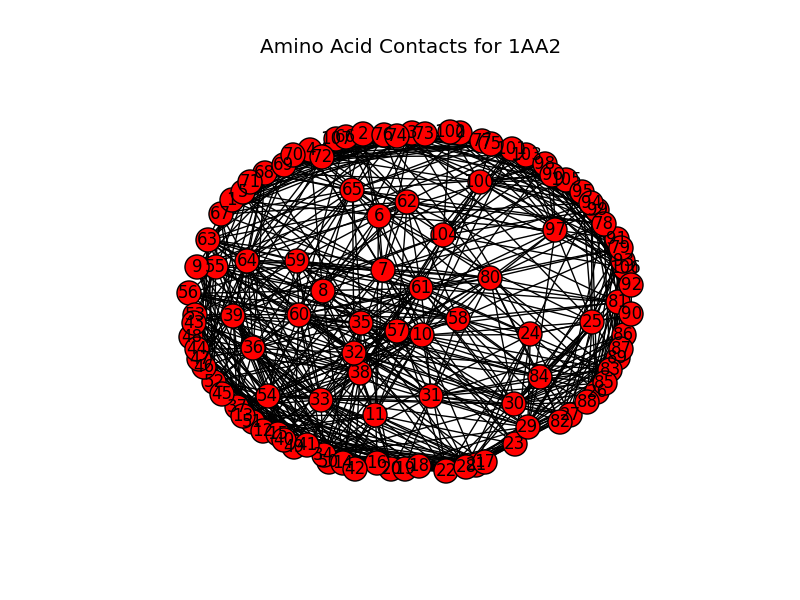
\includegraphics[scale=0.3]{1aa2_plot.png}
%\caption{Amino Acid Contact graph for Protein 1AA2.}
%\label{fig:contactgraph}
%\end{figure}
 
We observe that for this protein, most edges are highly localized among adjacent amino acids. However, many edges have connections across the protein, which is in and of itself an indicator of protein fold structure. We also observe that this graph is relatively sparse (compared to the complete graph), with 882 edges connecting 108 amino acids. 

\subsection{Model Results - ROC Curve}

% Final Results

%ROC CURVE

INSERT FIGURE HERE

The above figure displays the performance of the two models and a logistic baseline on a data set of N (CHANGE) training proteins, and M (CHANGE) test proteins. The ROC curve for  mean field learning is \textit{worse} than that of a random classifier, which has three possible implications for our model. The first is that there is some as-yet-undiscovered bug in our model code, leading to an error in calculating the gradient or log-likelihood that affects performance. The second is that gradient descent learning is getting stuck in a local optimum, leading to suboptimal results on test data. The third, and most likely, is that the mean field approximation is simply a poor approximation for this graph topology - modeling such a densely connected graph as fully disconnected ignores the graph topology and much of the effects of the triplet factors. The logistic classifier and the pseudo-log-likelihood model perform much better, although the pseudo-log-likelihood model performs similarly to the logistic classifier. A possible explanation is that the signal from the amino acid observations alone is not very strong, which hampers the effectiveness of the triplet factors and leads to the same performance. It is worth noting that the amino acid feature weights are always set to very low values in the mean field and pseudo-log-likelihood models (INSERT EXAMPLES HERE), indicating that the informational content of these features is low. While the amino acid pair may indicate pairing tendency within a single proteins, the general tendency of amino acids to be spatially close across multiple proteins is not very informative. This is clearly illustrated by the following contact maps, which show the relationship between amino acid pair distance and prediction. 

\subsection{Model Results - Individual Proteins}

IMAGE MAPS HERE
\begin{figure}
\centering
\begin{subfigure}{0.45\textwidth}
\includegraphics[width=\linewidth]{paper_images/true_adj.eps}
\centering
\caption{True adjacency matrix.}
\end{subfigure}
\begin{subfigure}{0.45\textwidth}
\includegraphics[width=\linewidth]{paper_images/logistic_adj.eps}
\centering
\caption{Logistic regression estimate.}
\end{subfigure}

\\

\begin{subfigure}{0.3\textwidth}
\includegraphics[width=\linewidth]{paper_images/pll_adj.eps}
\centering
\caption{Pseudo log-likelihood estimate}
\end{subfigure}
\end{figure}

IMAGE MAP DISCUSSION


\section{Conclusion and Future Work}


\begin{thebibliography}{9}
{\setlength\itemsep{0.0em}
\bibitem{wuyun16}
	Qiqige Wuyun, Wei Zheng, Zhenling Peng, and Jianyi Yang. November 1, 2016. A large-scale comparative assessment of methods for residue?residue contact prediction. Brief Bioinform (2016) doi:10.1093/bib/bbw106
\bibitem{colwell11}
	Debora S. Marks, Lucy J. Colwell, Robert Sheridan, Thomas A. Hopf, Andrea Pagnani, Riccardo Zecchina, Chris Sander. 25 October 2011. 3D Protein Structure Predicted from Sequence. {\tt arXiv:1110.5091 [q-bio.BM]}
\bibitem{ekeberg13}
	Magnus Ekeberg, Cecilia L{\"o}vkvist, Yueheng Lan, Martin Weigt, Erik Aurell. 12 January 2013. Improved contact prediction in proteins: Using pseudolikelihoods to infer Potts models. {\tt arXiv:1211.1281 [q-bio.QM]}
\bibitem{ma15}
	 Ma J., Wang S., Wang Z., Xu J. August 14, 2015. Protein contact prediction by integrating joint evolutionary coupling analysis and supervised learning. Bioinformatics 2015:btv472
\bibitem{wang16}
	Sheng Wang,  Wei Li, Renyu Zhang, Shiwang Liu and Jinbo Xu. April 12, 2016. CoinFold: a web server for protein contact prediction and contact-assisted protein folding. Nucl. Acids Res. (2016) doi: 10.1093/nar/gkw307
\bibitem{golkov16}
	Vladimir Golkov, Marcin J. Skwark, Antonij Golkov, Alexey Dosovitskiy, Thomas Brox, Jens Meiler, and Daniel Cremers. Protein contact prediction from amino acid co-evolution using convolutional networks for graph-valued images. In Proceedings of the 30th Conference on Neural Information Processing Systems (NIPS 2016), Barcelona, Spain.
%\bibitem{pdb}
%	H.M. Berman, J. Westbrook, Z. Feng, G. Gilliland, T.N. Bhat, H. Weissig, I.N. Shindyalov, P.E. Bourne. 2000. The Protein Data Bank
%Nucleic Acids Research, 28: 235-242.
}
\end{thebibliography}

\end{document}